\section{Introduction}
\label{sec:intro}

The use of Machine Learning in attempts to find new physics by probing High Energy Particle interactions has been ubiquitous, but unsupervised techiques are yet to find their place in this landscape. With vast volumes of data available from experiments like the Large Hadron Collider (LHC), it becomes increasingly desirable and ever more plausible that Unsupervised and Model-Free learning take a leading role in the hunt for new Physics.

Jet substructure is the analysis of radiation patterns and particle distributions within the collimated sprays of particles (jets) emerging from high-energy collisions. \cite{energyflow_poly}.
It has found a central importance in many of the searches for new physics at the Large Hadron Collider (LHC) and otherwise, some of them being:
\begin{itemize}
    \item Standard Model measurements
    \item Identification of boosted heavyparticles
    \item Discrimination of quark- from gluon- initiated jets
    \item Search of Beyond Standard Model particles
\end{itemize}

\subsection{Energy Flow Polynomials (EFPs)}

We have had several methods to represent jets as inputs to computational models, from a list of 4-vectors of constituent particles, to images of the jet itself amongst others, but either they are extremely sparse representations of the jets (as in the images) making is hard to ML models to learn something meaningful, or they have had an ordering (as in lists) not providing permutation invariance.

\begin{figure}
    \centering
    \begin{subfigure}[b]{0.49\textwidth}
        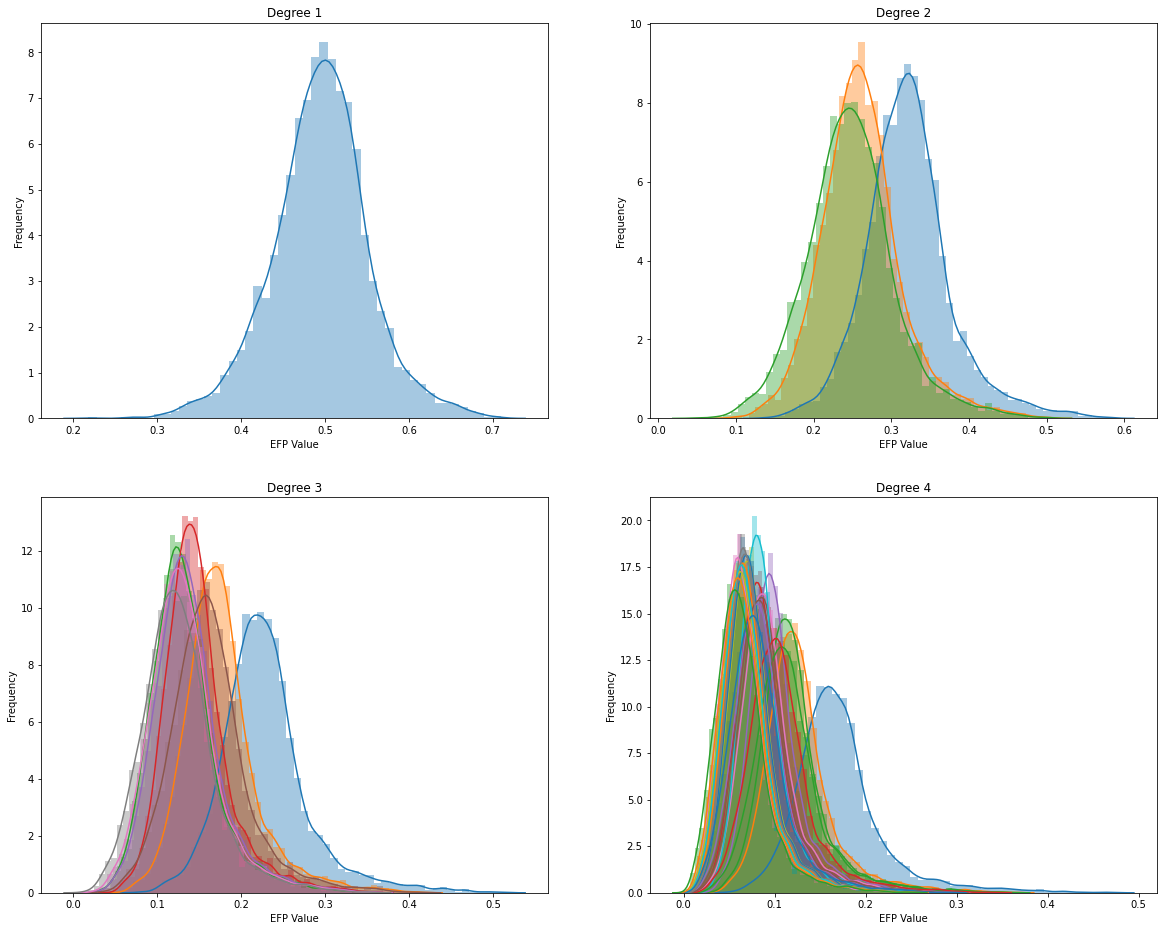
\includegraphics[width=\textwidth]{img/efp-qcd-particlenetdata.png}
        \caption{Histograms for QCD Jets}
    \end{subfigure}
    \begin{subfigure}[b]{0.49\textwidth}
        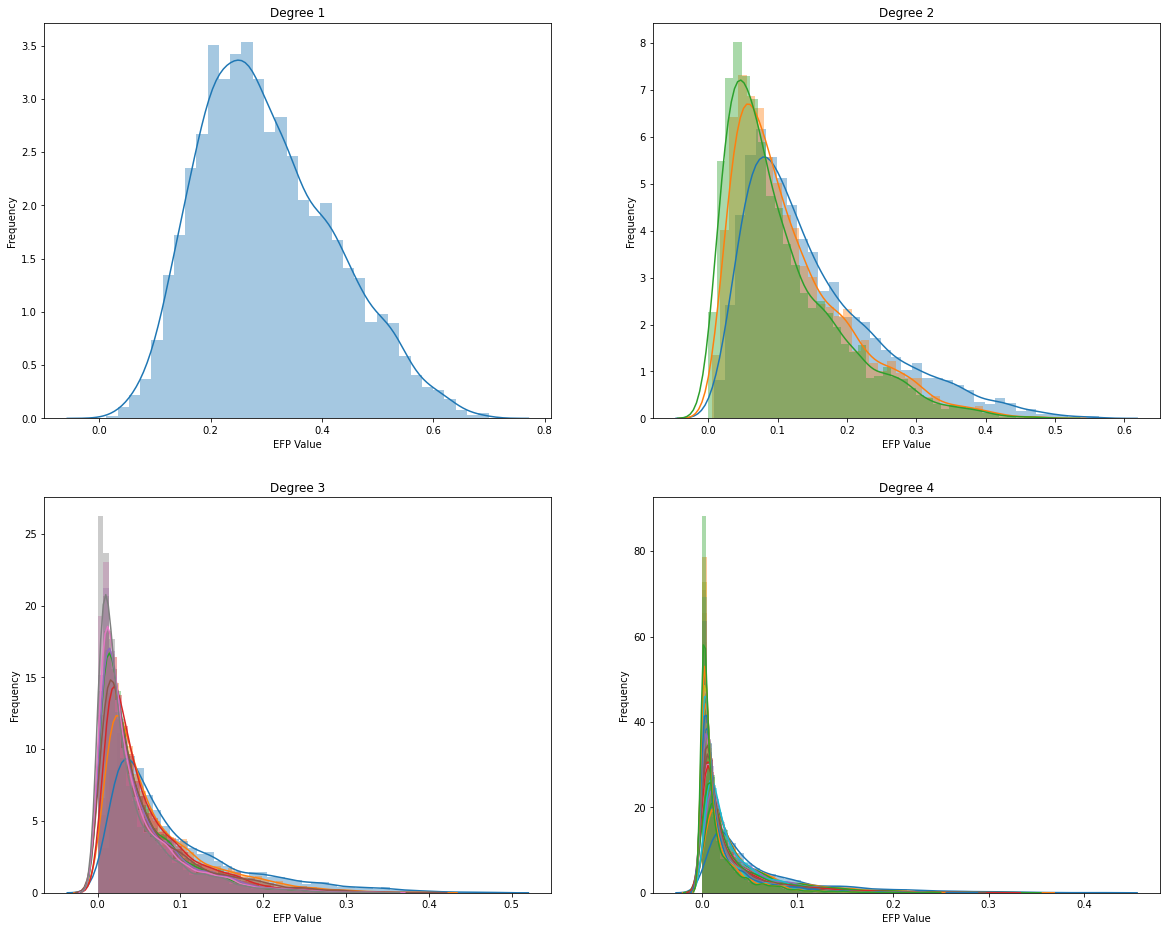
\includegraphics[width=\textwidth]{img/efp-top-particlenetdata.png}
        \caption{Histograms for Top Jets}
    \end{subfigure}
    \caption{EFP Polynomials on Top Tagging data}
    \label{fig:efp-histogram}
\end{figure}

\paragraph{EFPs as a method of jet representation} are both dense representations which inherently have permutation, as well as translational and rotational invariance. For any given jet, it's EFPs are Polynomials of the following form ~\cite{energyflow_poly}:
\begin{equation}
    \text{EFP}_{G} = \sum_{i_1 = 1}^{M} \dots \sum_{i_N = 1}^{M} z_{i_1} \dots z_{i_N} \prod_{k,l \in G} \theta_{i_k i_l}
\end{equation}
In addition, linear models trained on these polynomials perform nearly as well as the best Neural Networks on jet tagging tasks while having over an order magnitude fewer parameters. Owing to the fact that very simple supervised models can perform well using EFPs as the input representation, it seems natural that the same would apply to unsupervised techiniques.



\subsection{Latent Dirichet Allocation}

\textcolor{red}{Add details on what LDA does and any it's general issues, low accuracy, etc.}